\documentclass[11pt,a4paper,twocolumn]{article}
\usepackage[T1]{fontenc}
\usepackage[utf8]{inputenc}
\usepackage{anysize, longtable}
\usepackage{amsthm, amsfonts, amsmath, amssymb, booktabs, float}
\usepackage{sectsty, csquotes, xcolor, xspace, setspace, listings}
\usepackage{graphicx, tabularx, changepage, multirow, subcaption}
\usepackage{algorithm, algpseudocode, multicol, cuted, colortbl}
\usepackage{makecell, supertabular, stfloats}
\usepackage[hidelinks,bookmarksdepth=3]{hyperref}
\usepackage[capitalise]{cleveref}
\usepackage[inline]{enumitem}
\usepackage[english]{babel}
\usepackage{microtype}
\usepackage{libertinus}
\usepackage[scale = 0.85]{plex-mono}
\usepackage[maxbibnames=99]{biblatex}
\usepackage{titlesec}
\usepackage{tikz}

\usetikzlibrary{fit, shapes.geometric, positioning, shapes.misc, calc, arrows.meta, patterns, backgrounds, decorations, decorations.markings, decorations.pathreplacing, shadows, hobby}

\makeatletter

\thispagestyle{empty}

\theoremstyle{plain}
\newtheorem{theorem}{Theorem}
\newtheorem{lemma}{Lemma}

\theoremstyle{definition}
\newtheorem{definition}{Definition}
\newtheorem{example}{Example}

\theoremstyle{remark}
\newtheorem*{note}{Note}
\newtheorem*{remark}{Remark}

\newcommand{\inlinecode}[1]{\lstinline[basicstyle=\ttfamily,columns=fixed]$#1$}
\lstset{basicstyle=\setstretch{0}\small\ttfamily,breaklines=true,columns=fixed,captionpos=b,xleftmargin=0.5cm}

\newlength{\offsetpage}
\newenvironment{widepage}[1][2cm]{
  \setlength{\offsetpage}{#1}
  \begin{adjustwidth}{-\offsetpage}{-\offsetpage}
  \addtolength{\linewidth}{2\offsetpage}
}{\end{adjustwidth}}

\algnewcommand{\IIf}[1]{\State \algorithmicif\ #1\ \algorithmicthen}
\algnewcommand{\IElse}[1]{\algorithmicelse\ #1}
\algnewcommand{\EndIIf}{\unskip\ \algorithmicend\ \algorithmicif}

\addbibresource{biblio.bib}

\allowdisplaybreaks
\marginsize{2.0cm}{2.0cm}{1.25cm}{1.25cm}
\setcounter{tocdepth}{2}
\setlist[itemize]{topsep=0pt, partopsep=0pt, parsep=0pt, itemsep=\parskip}
\setlist[enumerate]{topsep=0pt, partopsep=0pt, parsep=0pt, itemsep=\parskip}
\titlespacing*{\section}{0pt}{0.5\baselineskip}{0.1\baselineskip}
\titlespacing*{\subsection}{0pt}{0.4\baselineskip}{0.1\baselineskip}
\titlespacing*{\subsubsection}{0pt}{0.3\baselineskip}{0.1\baselineskip}
\titlespacing*{\paragraph}{0pt}{0pt}{0.5\baselineskip}
\hbadness=10000

\title{Real-Time Analysis of Public GitHub Activity}
\author{Roland Bernard, 19598, \inlinecode{rolbernard@unibz.it}}
\date{August 2025}

\def\maketitle{
\begin{strip}
  \begin{adjustwidth}{5mm}{5mm}
    \vspace{-4.5em}
    \noindent{\small\bfseries Project Proposal\par}
    \vskip 0.25em
    \noindent{\LARGE\bfseries \@title\par}
    \vskip 1em
    \noindent{\large \@author\par}
    \vskip 1em
    \noindent{\small \@date\par}
    \vskip 1em
  \end{adjustwidth}
\end{strip}
}
\renewenvironment{abstract}{
  \vskip 1em
  \begin{quote}
  {\normalsize \abstractname\par}
  \small
}{
  \end{quote}
  \vskip 1em
}

\makeatother

\definecolor{unibzblue}{HTML}{0086ec}
\definecolor{unibzblue2}{HTML}{f0f8ff}

\pgfdeclarelayer{background}
\pgfdeclarelayer{foreground}
\pgfsetlayers{background,main,foreground}

\tikzset{
  flow/.style={-{Triangle[length=6, width=6]}, draw=red!70!black, very thick, shorten >= -3},
  biflow/.style={flow, {Triangle[length=6, width=6]}-{Triangle[length=6, width=6]}},
  link/.style={->, draw},
  ptr/.style={->, dashed},
  leafl/.style={-, thick},
  external/.style={inner sep=10, draw=black, fill=brown!20},
  internal/.style={inner sep=10, draw=black, fill=unibzblue!20},
  build/.style={inner sep=10, draw=black, fill=unibzblue!40},
  mixed/.style={inner sep=8.7, draw=black, path picture={
    \fill[brown!20] (path picture bounding box.south west)
      rectangle ($(path picture bounding box.north west)!.675!(path picture bounding box.north east)$);
    \fill[unibzblue!40] ($(path picture bounding box.north west)!.675!(path picture bounding box.north east)$)
      rectangle (path picture bounding box.south east);
  }},
  >=Latex, node distance=1, every node/.style={inner sep=0}
}


\begin{document}

\maketitle

\section{Application Domain} \label{application}

This project's goal is to develop an application for monitoring public activity on GitHub. GitHub is a large software development platform hosting many open source projects. The application will capture and analyze a continuous stream of public events to provide insights into ongoing open source development trends. The events to be analyzed include the creation of new repositories, branches, and forks; pushes to public repositories; the opening and closing of issues or pull requests; and the starring of repositories. The application will offer a live dashboard that visualizes the data, by processing it in real-time.

\section{Data Sources} \label{datasources}

The primary data source for this project will be the official \href{https://docs.github.com/en/rest/activity/events}{GitHub Events API}\footnote{\url{https://docs.github.com/en/rest/activity/events}}. Specifically, the project will use the \inlinecode{api.github.com/events} endpoint, which provides the most recent events across the entire platform. Each event is delivered as a JSON object containing detailed information about the action performed. By periodically polling this endpoint, we can obtain a high-volume stream of events.

\section{Technology and Architecture} \label{technology}

The system will be built using a variation of the provided reference architecture, as can be seen in \cref{fig:arch}.

\paragraph{Data Ingestion}
A Java-based Kafka Producer will be developed to poll the GitHub Events API. This component will handle de-duplication of events before publishing them as JSON to a dedicated Kafka topic.

\paragraph{Stream Processing}
Apache Flink will be used for stream processing. It will consume the raw event stream from Kafka and execute a series of computations, to derive meaningful analytics.

\paragraph{Data Serving}
The processed data from Flink will be published to new Kafka topics. A Java-based server will consume these topics and expose the results via a WebSocket connection to the frontend.

\paragraph{Frontend}
The user interface will be a custom single-page application using HTML and JavaScript, served by the frontend server. It will leverage the ECharts library to create an interactive dashboard with dynamic charts that update in real-time as new data arrives.

\begin{figure*}[ht]
  \centering
  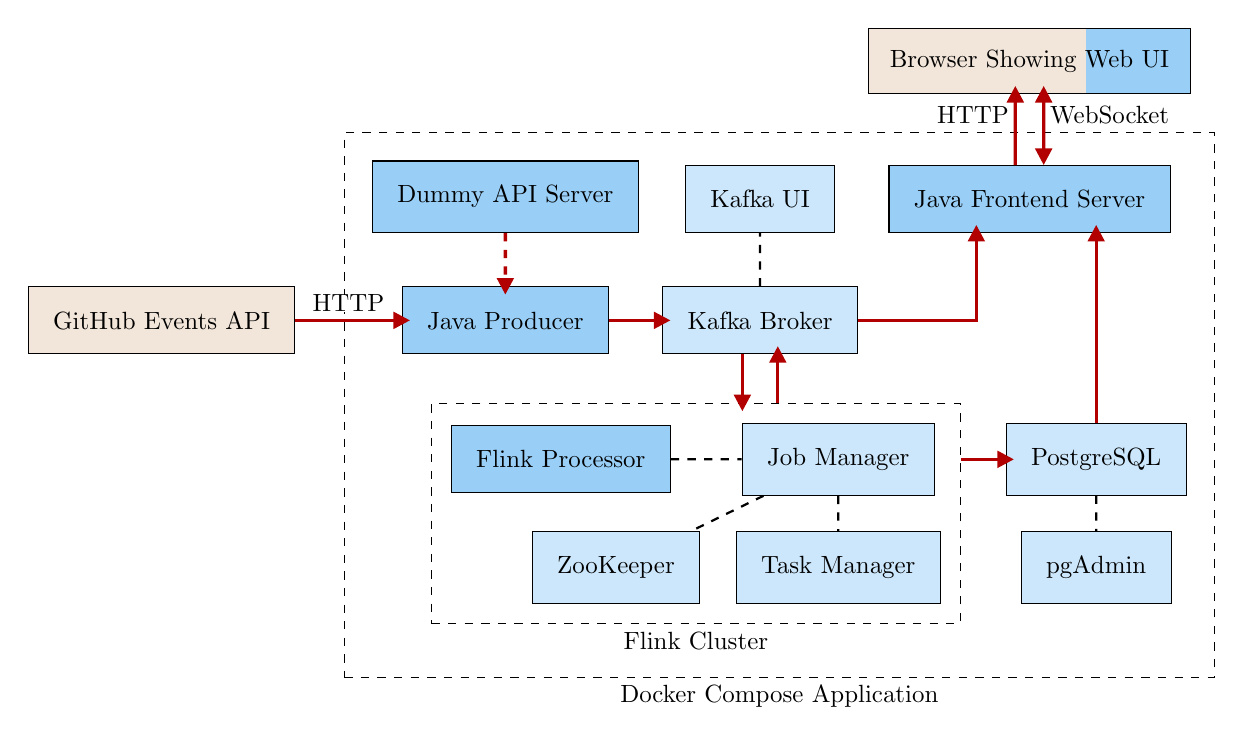
\begin{tikzpicture}[scale=0.9, transform shape]
    \node[external] (github) {GitHub Events API};
    \node[build, right=1.5 of github] (producer) {Java Producer};
    \draw[flow] (github) -> (producer) node [midway, fill=white, above=0.1] {HTTP};
    \node[internal, right=0.75 of producer] (kafka) {Kafka Broker};
    \draw[flow] (producer) -> (kafka);
    \node[internal, above=0.75 of kafka] (kafkaui) {Kafka UI};
    \draw[dashed, thick] (kafka) -> (kafkaui);
    \node[build, below=of kafka, xshift=-80] (processor) {Flink Processor};
    \node[internal, right=of processor] (jobmanager) {Job Manager};
    \draw[dashed, thick] (processor) -> (jobmanager);
    \node[internal, below=0.5 of jobmanager] (taskmanager) {Task Manager};
    \draw[dashed, thick] (jobmanager) -> (taskmanager);
    \node[internal, left=0.5 of taskmanager] (zookeeper) {ZooKeeper};
    \draw[dashed, thick] (jobmanager) -> (zookeeper);
    \begin{scope}[on background layer]
      \node[draw, dashed, fit=(processor)(jobmanager)(taskmanager), inner sep=7] (flink) {};
      \node[below=0.1 of flink] (flinklabel) {Flink Cluster};
    \end{scope}
    \draw[flow] ($(kafka.south)-(0.25,0)$) -> ($(kafka |- flink.north)-(0.25,0)$);
    \draw[flow] ($(kafka |- flink.north)+(0.25,0)$) -> ($(kafka.south)+(0.25,0)$);
    \node[build, above=0.75 of producer] (dummy) {Dummy API Server};
    \draw[flow, dashed] (dummy) -> (producer);
    \node[build, right=0.75 of kafkaui] (frontend) {Java Frontend Server};
    \draw[flow] (kafka) -| ($(frontend.south)-(0.75,0)$);
    \node[internal, right=of jobmanager] (postgres) {PostgreSQL};
    \node[internal, below=0.5 of postgres] (pgadmin) {pgAdmin};
    \draw[dashed, thick] (postgres) -- (pgadmin);
    \draw[flow] ($(postgres -| flink.east)$) -> ($(postgres.west)$);
    \draw[flow] ($(postgres.north)$) -> ($(postgres |- frontend.south)$);
    \node[mixed, above=of frontend] (browser) {Browser Showing Web UI};
    \draw[flow] ($(frontend.north)-(0.2,0)$) -> ($(browser.south)-(0.2,0)$) node [midway, fill=white, above left=0.1] {HTTP};
    \draw[biflow] ($(frontend.north)+(0.2,0)$) -> ($(browser.south)+(0.2,0)$) node [midway, fill=white, above right=0.1] {WebSocket};
    \begin{scope}[on background layer]
      \node[draw, dashed, fit=(flink)(flinklabel)(producer)(kafkaui)(frontend)(dummy)(postgres), inner sep=10] (docker) {};
      \node[below=0.1 of docker] (dockerlabel) {Docker Compose Application};
    \end{scope}
  \end{tikzpicture}
  \caption{Implemented application architecture. Blue indicates parts of the architecture controlled by the project, while the brown indicates external components. Darker blue represents components implemented as part of the project, while light blue components represent the use of existing software that has merely been configured.}
  \label{fig:arch}
\end{figure*}


\section{Functionalities} \label{functionalities}

The project will provide several features on the frontend dashboard:

\paragraph{Live Event Feed}
A filterable, real-time stream of raw events, allowing users to filter based on event type, username, or repository name.

\paragraph{Real-Time Event Counters}
Dynamic counters displaying the volume of different event types (e.g., commits, issues opened, forks, etc.) over sliding time windows, such as the last minute, 5 minutes, or hour.

\paragraph{Activity Leaderboards}
Continuously updated rankings of the most active repositories and users. This will be calculated based on the number of events over a sliding time window, such as the last 2 hours.

\paragraph{Trending Repository Detection}
Identification of repositories that are rapidly gaining popularity. This will be achieved by analyzing the rate of new stars. Flink will calculate the rate of new stars over time, allowing the system to flag repositories experiencing a significant increase in interest.

\end{document}
